\documentclass[1p]{elsarticle_modified}
%\bibliographystyle{elsarticle-num}

%\usepackage[colorlinks]{hyperref}
%\usepackage{abbrmath_seonhwa} %\Abb, \Ascr, \Acal ,\Abf, \Afrak
\usepackage{amsfonts}
\usepackage{amssymb}
\usepackage{amsmath}
\usepackage{amsthm}
\usepackage{scalefnt}
\usepackage{amsbsy}
\usepackage{kotex}
\usepackage{caption}
\usepackage{subfig}
\usepackage{color}
\usepackage{graphicx}
\usepackage{xcolor} %% white, black, red, green, blue, cyan, magenta, yellow
\usepackage{float}
\usepackage{setspace}
\usepackage{hyperref}

\usepackage{tikz}
\usetikzlibrary{arrows}

\usepackage{multirow}
\usepackage{array} % fixed length table
\usepackage{hhline}

%%%%%%%%%%%%%%%%%%%%%
\makeatletter
\renewcommand*\env@matrix[1][\arraystretch]{%
	\edef\arraystretch{#1}%
	\hskip -\arraycolsep
	\let\@ifnextchar\new@ifnextchar
	\array{*\c@MaxMatrixCols c}}
\makeatother %https://tex.stackexchange.com/questions/14071/how-can-i-increase-the-line-spacing-in-a-matrix
%%%%%%%%%%%%%%%

\usepackage[normalem]{ulem}

\newcommand{\msout}[1]{\ifmmode\text{\sout{\ensuremath{#1}}}\else\sout{#1}\fi}
%SOURCE: \msout is \stkout macro in https://tex.stackexchange.com/questions/20609/strikeout-in-math-mode

\newcommand{\cancel}[1]{
	\ifmmode
	{\color{red}\msout{#1}}
	\else
	{\color{red}\sout{#1}}
	\fi
}

\newcommand{\add}[1]{
	{\color{blue}\uwave{#1}}
}

\newcommand{\replace}[2]{
	\ifmmode
	{\color{red}\msout{#1}}{\color{blue}\uwave{#2}}
	\else
	{\color{red}\sout{#1}}{\color{blue}\uwave{#2}}
	\fi
}

\newcommand{\Sol}{\mathcal{S}} %segment
\newcommand{\D}{D} %diagram
\newcommand{\A}{\mathcal{A}} %arc


%%%%%%%%%%%%%%%%%%%%%%%%%%%%%5 test

\def\sl{\operatorname{\textup{SL}}(2,\Cbb)}
\def\psl{\operatorname{\textup{PSL}}(2,\Cbb)}
\def\quan{\mkern 1mu \triangleright \mkern 1mu}

\theoremstyle{definition}
\newtheorem{thm}{Theorem}[section]
\newtheorem{prop}[thm]{Proposition}
\newtheorem{lem}[thm]{Lemma}
\newtheorem{ques}[thm]{Question}
\newtheorem{cor}[thm]{Corollary}
\newtheorem{defn}[thm]{Definition}
\newtheorem{exam}[thm]{Example}
\newtheorem{rmk}[thm]{Remark}
\newtheorem{alg}[thm]{Algorithm}

\newcommand{\I}{\sqrt{-1}}
\begin{document}

%\begin{frontmatter}
%
%\title{Boundary parabolic representations of knots up to 8 crossings}
%
%%% Group authors per affiliation:
%\author{Yunhi Cho} 
%\address{Department of Mathematics, University of Seoul, Seoul, Korea}
%\ead{yhcho@uos.ac.kr}
%
%
%\author{Seonhwa Kim} %\fnref{s_kim}}
%\address{Center for Geometry and Physics, Institute for Basic Science, Pohang, 37673, Korea}
%\ead{ryeona17@ibs.re.kr}
%
%\author{Hyuk Kim}
%\address{Department of Mathematical Sciences, Seoul National University, Seoul 08826, Korea}
%\ead{hyukkim@snu.ac.kr}
%
%\author{Seokbeom Yoon}
%\address{Department of Mathematical Sciences, Seoul National University, Seoul, 08826,  Korea}
%\ead{sbyoon15@snu.ac.kr}
%
%\begin{abstract}
%We find all boundary parabolic representation of knots up to 8 crossings.
%
%\end{abstract}
%\begin{keyword}
%    \MSC[2010] 57M25 
%\end{keyword}
%
%\end{frontmatter}

%\linenumbers
%\tableofcontents
%
\newcommand\colored[1]{\textcolor{white}{\rule[-0.35ex]{0.8em}{1.4ex}}\kern-0.8em\color{red} #1}%
%\newcommand\colored[1]{\textcolor{white}{ #1}\kern-2.17ex	\textcolor{white}{ #1}\kern-1.81ex	\textcolor{white}{ #1}\kern-2.15ex\color{red}#1	}

{\Large $\underline{11a_{178}~(K11a_{178})}$}

\setlength{\tabcolsep}{10pt}
\renewcommand{\arraystretch}{1.6}
\vspace{1cm}\begin{tabular}{m{100pt}>{\centering\arraybackslash}m{274pt}}
\multirow{5}{120pt}{
	\centering
	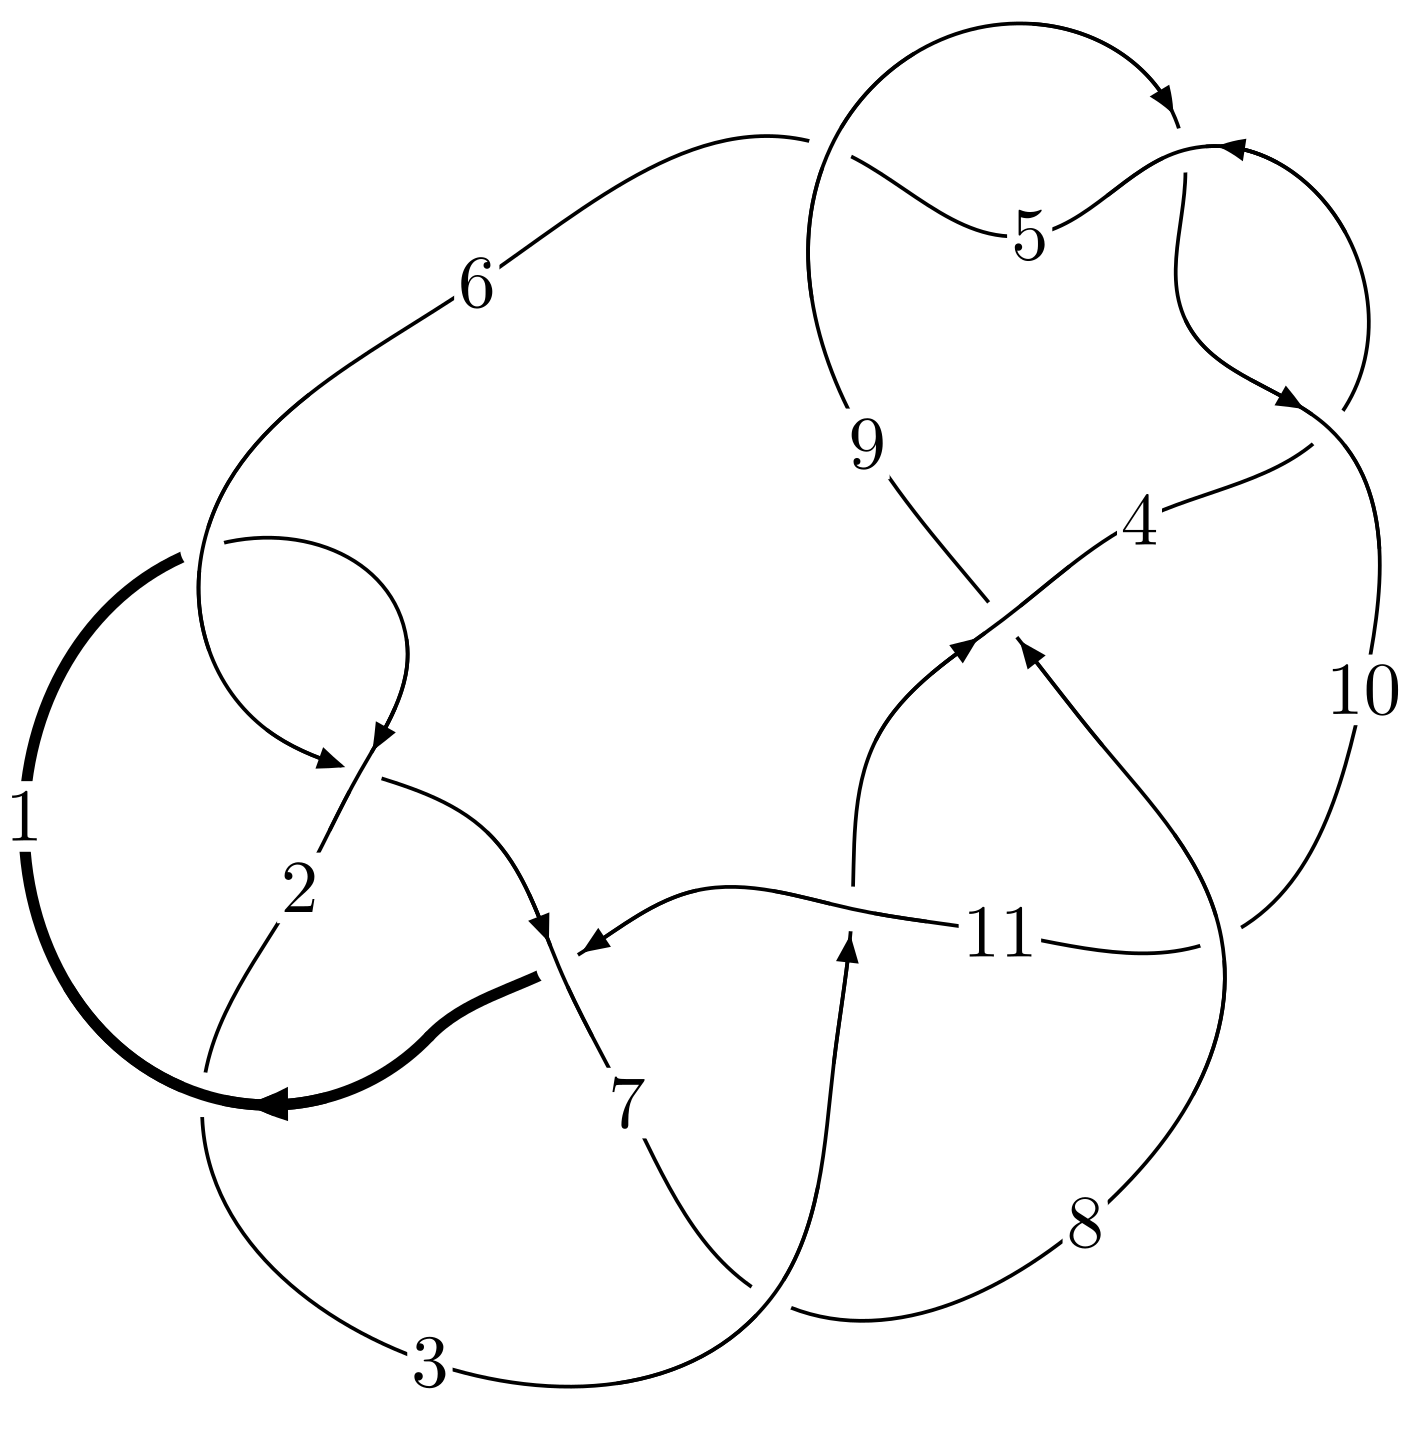
\includegraphics[width=112pt]{../../../GIT/diagram.site/Diagrams/png/427_11a_178.png}\\
\ \ \ A knot diagram\footnotemark}&
\allowdisplaybreaks
\textbf{Linearized knot diagam} \\
\cline{2-2}
 &
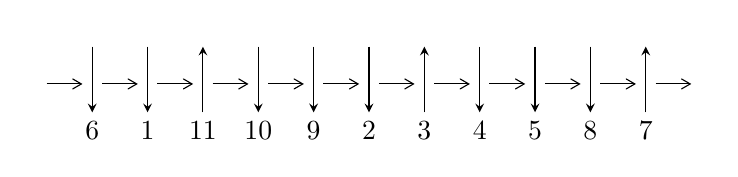
\begin{tikzpicture}[x=20pt, y=17pt]
	% nodes
	\node (C0) at (0, 0) {};
	\node (C1) at (1, 0) {};
	\node (C1U) at (1, +1) {};
	\node (C1D) at (1, -1) {6};

	\node (C2) at (2, 0) {};
	\node (C2U) at (2, +1) {};
	\node (C2D) at (2, -1) {1};

	\node (C3) at (3, 0) {};
	\node (C3U) at (3, +1) {};
	\node (C3D) at (3, -1) {11};

	\node (C4) at (4, 0) {};
	\node (C4U) at (4, +1) {};
	\node (C4D) at (4, -1) {10};

	\node (C5) at (5, 0) {};
	\node (C5U) at (5, +1) {};
	\node (C5D) at (5, -1) {9};

	\node (C6) at (6, 0) {};
	\node (C6U) at (6, +1) {};
	\node (C6D) at (6, -1) {2};

	\node (C7) at (7, 0) {};
	\node (C7U) at (7, +1) {};
	\node (C7D) at (7, -1) {3};

	\node (C8) at (8, 0) {};
	\node (C8U) at (8, +1) {};
	\node (C8D) at (8, -1) {4};

	\node (C9) at (9, 0) {};
	\node (C9U) at (9, +1) {};
	\node (C9D) at (9, -1) {5};

	\node (C10) at (10, 0) {};
	\node (C10U) at (10, +1) {};
	\node (C10D) at (10, -1) {8};

	\node (C11) at (11, 0) {};
	\node (C11U) at (11, +1) {};
	\node (C11D) at (11, -1) {7};
	\node (C12) at (12, 0) {};

	% arrows
	\draw[->,>={angle 60}]
	(C0) edge (C1) (C1) edge (C2) (C2) edge (C3) (C3) edge (C4) (C4) edge (C5) (C5) edge (C6) (C6) edge (C7) (C7) edge (C8) (C8) edge (C9) (C9) edge (C10) (C10) edge (C11) (C11) edge (C12) ;	\draw[->,>=stealth]
	(C1U) edge (C1D) (C2U) edge (C2D) (C3D) edge (C3U) (C4U) edge (C4D) (C5U) edge (C5D) (C6U) edge (C6D) (C7D) edge (C7U) (C8U) edge (C8D) (C9U) edge (C9D) (C10U) edge (C10D) (C11D) edge (C11U) ;
	\end{tikzpicture} \\
\hhline{~~} \\& 
\textbf{Solving Sequence} \\ \cline{2-2} 
 &
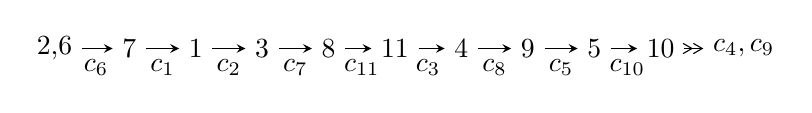
\begin{tikzpicture}[x=24pt, y=7pt]
	% node
	\node (A0) at (-1/8, 0) {2,6};
	\node (A1) at (1, 0) {7};
	\node (A2) at (2, 0) {1};
	\node (A3) at (3, 0) {3};
	\node (A4) at (4, 0) {8};
	\node (A5) at (5, 0) {11};
	\node (A6) at (6, 0) {4};
	\node (A7) at (7, 0) {9};
	\node (A8) at (8, 0) {5};
	\node (A9) at (9, 0) {10};
	\node (C1) at (1/2, -1) {$c_{6}$};
	\node (C2) at (3/2, -1) {$c_{1}$};
	\node (C3) at (5/2, -1) {$c_{2}$};
	\node (C4) at (7/2, -1) {$c_{7}$};
	\node (C5) at (9/2, -1) {$c_{11}$};
	\node (C6) at (11/2, -1) {$c_{3}$};
	\node (C7) at (13/2, -1) {$c_{8}$};
	\node (C8) at (15/2, -1) {$c_{5}$};
	\node (C9) at (17/2, -1) {$c_{10}$};
	\node (A10) at (41/4, 0) {$c_{4},c_{9}$};

	% edge
	\draw[->,>=stealth]	
	(A0) edge (A1) (A1) edge (A2) (A2) edge (A3) (A3) edge (A4) (A4) edge (A5) (A5) edge (A6) (A6) edge (A7) (A7) edge (A8) (A8) edge (A9) ;
	\draw[->>,>={angle 60}]	
	(A9) edge (A10);
\end{tikzpicture} \\ 

\end{tabular} \\

\footnotetext{
The image of knot diagram is generated by the software ``\textbf{Draw programme}" developed by Andrew Bartholomew(\url{http://www.layer8.co.uk/maths/draw/index.htm\#Running-draw}), where we modified some parts for our purpose(\url{https://github.com/CATsTAILs/LinksPainter}).
}\phantom \\ \newline 
\centering \textbf{Ideals for irreducible components\footnotemark of $X_{\text{par}}$} 
 
\begin{align*}
I^u_{1}&=\langle 
u^{61}- u^{60}+\cdots- u+1\rangle \\
\\
\end{align*}
\raggedright * 1 irreducible components of $\dim_{\mathbb{C}}=0$, with total 61 representations.\\
\footnotetext{All coefficients of polynomials are rational numbers. But the coefficients are sometimes approximated in decimal forms when there is not enough margin.}
\newpage
\renewcommand{\arraystretch}{1}
\centering \section*{I. $I^u_{1}= \langle u^{61}- u^{60}+\cdots- u+1 \rangle$}
\flushleft \textbf{(i) Arc colorings}\\
\begin{tabular}{m{7pt} m{180pt} m{7pt} m{180pt} }
\flushright $a_{2}=$&$\begin{pmatrix}0\\u\end{pmatrix}$ \\
\flushright $a_{6}=$&$\begin{pmatrix}1\\0\end{pmatrix}$ \\
\flushright $a_{7}=$&$\begin{pmatrix}1\\u^2\end{pmatrix}$ \\
\flushright $a_{1}=$&$\begin{pmatrix}u\\u\end{pmatrix}$ \\
\flushright $a_{3}=$&$\begin{pmatrix}- u^3\\- u^3+u\end{pmatrix}$ \\
\flushright $a_{8}=$&$\begin{pmatrix}u^8- u^6+u^4+1\\u^8-2 u^6+2 u^4\end{pmatrix}$ \\
\flushright $a_{11}=$&$\begin{pmatrix}u^3\\u^5- u^3+u\end{pmatrix}$ \\
\flushright $a_{4}=$&$\begin{pmatrix}u^{11}-2 u^9+2 u^7- u^3\\u^{13}-3 u^{11}+5 u^9-4 u^7+2 u^5- u^3+u\end{pmatrix}$ \\
\flushright $a_{9}=$&$\begin{pmatrix}u^{32}-7 u^{30}+\cdots+2 u^{12}+1\\u^{34}-8 u^{32}+\cdots+4 u^6+u^2\end{pmatrix}$ \\
\flushright $a_{5}=$&$\begin{pmatrix}- u^{55}+12 u^{53}+\cdots-5 u^7-2 u^3\\- u^{55}+13 u^{53}+\cdots-2 u^3+u\end{pmatrix}$ \\
\flushright $a_{10}=$&$\begin{pmatrix}u^{21}-4 u^{19}+9 u^{17}-12 u^{15}+12 u^{13}-10 u^{11}+9 u^9-6 u^7+3 u^5+u\\u^{21}-5 u^{19}+13 u^{17}-20 u^{15}+20 u^{13}-13 u^{11}+7 u^9-4 u^7+3 u^5- u^3+u\end{pmatrix}$\\ \flushright $a_{10}=$&$\begin{pmatrix}u^{21}-4 u^{19}+9 u^{17}-12 u^{15}+12 u^{13}-10 u^{11}+9 u^9-6 u^7+3 u^5+u\\u^{21}-5 u^{19}+13 u^{17}-20 u^{15}+20 u^{13}-13 u^{11}+7 u^9-4 u^7+3 u^5- u^3+u\end{pmatrix}$\\&\end{tabular}
\flushleft \textbf{(ii) Obstruction class $= -1$}\\~\\
\flushleft \textbf{(iii) Cusp Shapes $= 4 u^{59}-56 u^{57}+\cdots+8 u-2$}\\~\\
\newpage\renewcommand{\arraystretch}{1}
\flushleft \textbf{(iv) u-Polynomials at the component}\newline \\
\begin{tabular}{m{50pt}|m{274pt}}
Crossings & \hspace{64pt}u-Polynomials at each crossing \\
\hline $$\begin{aligned}c_{1},c_{6}\end{aligned}$$&$\begin{aligned}
&u^{61}- u^{60}+\cdots- u+1
\end{aligned}$\\
\hline $$\begin{aligned}c_{2}\end{aligned}$$&$\begin{aligned}
&u^{61}+29 u^{60}+\cdots+3 u+1
\end{aligned}$\\
\hline $$\begin{aligned}c_{3}\end{aligned}$$&$\begin{aligned}
&u^{61}+7 u^{60}+\cdots+433 u+37
\end{aligned}$\\
\hline $$\begin{aligned}c_{4},c_{5},c_{9}\end{aligned}$$&$\begin{aligned}
&u^{61}+u^{60}+\cdots+3 u+1
\end{aligned}$\\
\hline $$\begin{aligned}c_{7}\end{aligned}$$&$\begin{aligned}
&u^{61}+u^{60}+\cdots-211 u+61
\end{aligned}$\\
\hline $$\begin{aligned}c_{8}\end{aligned}$$&$\begin{aligned}
&u^{61}- u^{60}+\cdots+11 u+2
\end{aligned}$\\
\hline $$\begin{aligned}c_{10}\end{aligned}$$&$\begin{aligned}
&u^{61}-13 u^{60}+\cdots-3083 u+283
\end{aligned}$\\
\hline $$\begin{aligned}c_{11}\end{aligned}$$&$\begin{aligned}
&u^{61}-3 u^{60}+\cdots-89 u+56
\end{aligned}$\\
\hline
\end{tabular}\\~\\
\newpage\renewcommand{\arraystretch}{1}
\flushleft \textbf{(v) Riley Polynomials at the component}\newline \\
\begin{tabular}{m{50pt}|m{274pt}}
Crossings & \hspace{64pt}Riley Polynomials at each crossing \\
\hline $$\begin{aligned}c_{1},c_{6}\end{aligned}$$&$\begin{aligned}
&y^{61}-29 y^{60}+\cdots+3 y-1
\end{aligned}$\\
\hline $$\begin{aligned}c_{2}\end{aligned}$$&$\begin{aligned}
&y^{61}+7 y^{60}+\cdots- y-1
\end{aligned}$\\
\hline $$\begin{aligned}c_{3}\end{aligned}$$&$\begin{aligned}
&y^{61}+11 y^{60}+\cdots-18009 y-1369
\end{aligned}$\\
\hline $$\begin{aligned}c_{4},c_{5},c_{9}\end{aligned}$$&$\begin{aligned}
&y^{61}+55 y^{60}+\cdots+3 y-1
\end{aligned}$\\
\hline $$\begin{aligned}c_{7}\end{aligned}$$&$\begin{aligned}
&y^{61}-13 y^{60}+\cdots+176159 y-3721
\end{aligned}$\\
\hline $$\begin{aligned}c_{8}\end{aligned}$$&$\begin{aligned}
&y^{61}+3 y^{60}+\cdots+57 y-4
\end{aligned}$\\
\hline $$\begin{aligned}c_{10}\end{aligned}$$&$\begin{aligned}
&y^{61}+19 y^{60}+\cdots-760653 y-80089
\end{aligned}$\\
\hline $$\begin{aligned}c_{11}\end{aligned}$$&$\begin{aligned}
&y^{61}+15 y^{60}+\cdots-75183 y-3136
\end{aligned}$\\
\hline
\end{tabular}\\~\\
\newpage\flushleft \textbf{(vi) Complex Volumes and Cusp Shapes}
$$\begin{array}{c|c|c}  
\text{Solutions to }I^u_{1}& \I (\text{vol} + \sqrt{-1}CS) & \text{Cusp shape}\\
 \hline 
\begin{aligned}
u &= \phantom{-}1.033100 + 0.187577 I\end{aligned}
 & \phantom{-}3.27959 - 1.47237 I & -3.77294 + 0.98684 I \\ \hline\begin{aligned}
u &= \phantom{-}1.033100 - 0.187577 I\end{aligned}
 & \phantom{-}3.27959 + 1.47237 I & -3.77294 - 0.98684 I \\ \hline\begin{aligned}
u &= \phantom{-}0.621785 + 0.658999 I\end{aligned}
 & \phantom{-}7.14477 - 7.36689 I & \phantom{-}1.83265 + 6.49541 I \\ \hline\begin{aligned}
u &= \phantom{-}0.621785 - 0.658999 I\end{aligned}
 & \phantom{-}7.14477 + 7.36689 I & \phantom{-}1.83265 - 6.49541 I \\ \hline\begin{aligned}
u &= -0.957071 + 0.545546 I\end{aligned}
 & \phantom{-}0.605205 + 0.585495 I & -3.92457 + 0. I\phantom{ +0.000000I} \\ \hline\begin{aligned}
u &= -0.957071 - 0.545546 I\end{aligned}
 & \phantom{-}0.605205 - 0.585495 I & -3.92457 + 0. I\phantom{ +0.000000I} \\ \hline\begin{aligned}
u &= \phantom{-}0.948153 + 0.574834 I\end{aligned}
 & \phantom{-}6.18322 + 2.55917 I & \phantom{-0.000000 } 0 \\ \hline\begin{aligned}
u &= \phantom{-}0.948153 - 0.574834 I\end{aligned}
 & \phantom{-}6.18322 - 2.55917 I & \phantom{-0.000000 } 0 \\ \hline\begin{aligned}
u &= -0.612486 + 0.631132 I\end{aligned}
 & \phantom{-}1.61526 + 4.05129 I & -2.39277 - 6.82409 I \\ \hline\begin{aligned}
u &= -0.612486 - 0.631132 I\end{aligned}
 & \phantom{-}1.61526 - 4.05129 I & -2.39277 + 6.82409 I \\ \hline\begin{aligned}
u &= -1.089710 + 0.268806 I\end{aligned}
 & -2.65665 + 0.24134 I & -8.01162 + 0. I\phantom{ +0.000000I} \\ \hline\begin{aligned}
u &= -1.089710 - 0.268806 I\end{aligned}
 & -2.65665 - 0.24134 I & -8.01162 + 0. I\phantom{ +0.000000I} \\ \hline\begin{aligned}
u &= -0.541944 + 0.674012 I\end{aligned}
 & \phantom{-}8.48817 - 1.61774 I & \phantom{-}3.86252 + 0.20232 I \\ \hline\begin{aligned}
u &= -0.541944 - 0.674012 I\end{aligned}
 & \phantom{-}8.48817 + 1.61774 I & \phantom{-}3.86252 - 0.20232 I \\ \hline\begin{aligned}
u &= \phantom{-}1.003470 + 0.545968 I\end{aligned}
 & \phantom{-}1.15617 - 4.09014 I & \phantom{-0.000000 } 0 \\ \hline\begin{aligned}
u &= \phantom{-}1.003470 - 0.545968 I\end{aligned}
 & \phantom{-}1.15617 + 4.09014 I & \phantom{-0.000000 } 0 \\ \hline\begin{aligned}
u &= \phantom{-}1.120400 + 0.239796 I\end{aligned}
 & -4.20404 + 3.36287 I & \phantom{-0.000000 } 0 \\ \hline\begin{aligned}
u &= \phantom{-}1.120400 - 0.239796 I\end{aligned}
 & -4.20404 - 3.36287 I & \phantom{-0.000000 } 0 \\ \hline\begin{aligned}
u &= -1.129610 + 0.223326 I\end{aligned}
 & \phantom{-}1.12751 - 6.89407 I & \phantom{-0.000000 } 0 \\ \hline\begin{aligned}
u &= -1.129610 - 0.223326 I\end{aligned}
 & \phantom{-}1.12751 + 6.89407 I & \phantom{-0.000000 } 0 \\ \hline\begin{aligned}
u &= -1.112280 + 0.300936 I\end{aligned}
 & -2.83860 + 0.05729 I & \phantom{-0.000000 } 0 \\ \hline\begin{aligned}
u &= -1.112280 - 0.300936 I\end{aligned}
 & -2.83860 - 0.05729 I & \phantom{-0.000000 } 0 \\ \hline\begin{aligned}
u &= \phantom{-}0.702655 + 0.463134 I\end{aligned}
 & \phantom{-}2.64368 - 1.93405 I & -1.89634 + 4.21284 I \\ \hline\begin{aligned}
u &= \phantom{-}0.702655 - 0.463134 I\end{aligned}
 & \phantom{-}2.64368 + 1.93405 I & -1.89634 - 4.21284 I \\ \hline\begin{aligned}
u &= \phantom{-}0.343323 + 0.767640 I\end{aligned}
 & \phantom{-}5.74647 + 9.59086 I & \phantom{-}0.22395 - 6.02636 I \\ \hline\begin{aligned}
u &= \phantom{-}0.343323 - 0.767640 I\end{aligned}
 & \phantom{-}5.74647 - 9.59086 I & \phantom{-}0.22395 + 6.02636 I \\ \hline\begin{aligned}
u &= -1.010660 + 0.577213 I\end{aligned}
 & \phantom{-}7.10735 + 6.46891 I & \phantom{-0.000000 } 0 \\ \hline\begin{aligned}
u &= -1.010660 - 0.577213 I\end{aligned}
 & \phantom{-}7.10735 - 6.46891 I & \phantom{-0.000000 } 0 \\ \hline\begin{aligned}
u &= \phantom{-}1.115370 + 0.342685 I\end{aligned}
 & -5.28239 - 3.39079 I & \phantom{-0.000000 } 0 \\ \hline\begin{aligned}
u &= \phantom{-}1.115370 - 0.342685 I\end{aligned}
 & -5.28239 + 3.39079 I & \phantom{-0.000000 } 0\\
 \hline 
 \end{array}$$\newpage$$\begin{array}{c|c|c}  
\text{Solutions to }I^u_{1}& \I (\text{vol} + \sqrt{-1}CS) & \text{Cusp shape}\\
 \hline 
\begin{aligned}
u &= -0.394147 + 0.730677 I\end{aligned}
 & \phantom{-}7.77499 - 0.61886 I & \phantom{-}2.98419 + 0.41079 I \\ \hline\begin{aligned}
u &= -0.394147 - 0.730677 I\end{aligned}
 & \phantom{-}7.77499 + 0.61886 I & \phantom{-}2.98419 - 0.41079 I \\ \hline\begin{aligned}
u &= \phantom{-}0.552270 + 0.617769 I\end{aligned}
 & \phantom{-}2.48756 - 0.50881 I & \phantom{-}0.570526 - 0.185507 I \\ \hline\begin{aligned}
u &= \phantom{-}0.552270 - 0.617769 I\end{aligned}
 & \phantom{-}2.48756 + 0.50881 I & \phantom{-}0.570526 + 0.185507 I \\ \hline\begin{aligned}
u &= -0.336261 + 0.751744 I\end{aligned}
 & \phantom{-}0.27382 - 6.06188 I & -4.21507 + 6.02215 I \\ \hline\begin{aligned}
u &= -0.336261 - 0.751744 I\end{aligned}
 & \phantom{-}0.27382 + 6.06188 I & -4.21507 - 6.02215 I \\ \hline\begin{aligned}
u &= -1.124710 + 0.366091 I\end{aligned}
 & -0.41617 + 6.80603 I & \phantom{-0.000000 } 0 \\ \hline\begin{aligned}
u &= -1.124710 - 0.366091 I\end{aligned}
 & -0.41617 - 6.80603 I & \phantom{-0.000000 } 0 \\ \hline\begin{aligned}
u &= \phantom{-}0.345416 + 0.715523 I\end{aligned}
 & \phantom{-}1.53930 + 2.31744 I & -1.192371 - 0.636222 I \\ \hline\begin{aligned}
u &= \phantom{-}0.345416 - 0.715523 I\end{aligned}
 & \phantom{-}1.53930 - 2.31744 I & -1.192371 + 0.636222 I \\ \hline\begin{aligned}
u &= \phantom{-}1.113390 + 0.485777 I\end{aligned}
 & \phantom{-}0.382880 - 0.851377 I & \phantom{-0.000000 } 0 \\ \hline\begin{aligned}
u &= \phantom{-}1.113390 - 0.485777 I\end{aligned}
 & \phantom{-}0.382880 + 0.851377 I & \phantom{-0.000000 } 0 \\ \hline\begin{aligned}
u &= -1.112330 + 0.510589 I\end{aligned}
 & -4.14943 + 4.18449 I & \phantom{-0.000000 } 0 \\ \hline\begin{aligned}
u &= -1.112330 - 0.510589 I\end{aligned}
 & -4.14943 - 4.18449 I & \phantom{-0.000000 } 0 \\ \hline\begin{aligned}
u &= -1.096940 + 0.573191 I\end{aligned}
 & \phantom{-}5.71025 + 5.58980 I & \phantom{-0.000000 } 0 \\ \hline\begin{aligned}
u &= -1.096940 - 0.573191 I\end{aligned}
 & \phantom{-}5.71025 - 5.58980 I & \phantom{-0.000000 } 0 \\ \hline\begin{aligned}
u &= \phantom{-}1.118690 + 0.534112 I\end{aligned}
 & -1.26791 - 7.55537 I & \phantom{-0.000000 } 0 \\ \hline\begin{aligned}
u &= \phantom{-}1.118690 - 0.534112 I\end{aligned}
 & -1.26791 + 7.55537 I & \phantom{-0.000000 } 0 \\ \hline\begin{aligned}
u &= \phantom{-}1.111260 + 0.557520 I\end{aligned}
 & -0.69264 - 7.18756 I & \phantom{-0.000000 } 0 \\ \hline\begin{aligned}
u &= \phantom{-}1.111260 - 0.557520 I\end{aligned}
 & -0.69264 + 7.18756 I & \phantom{-0.000000 } 0 \\ \hline\begin{aligned}
u &= \phantom{-}0.277033 + 0.691934 I\end{aligned}
 & \phantom{-}1.13938 + 2.86125 I & -3.45602 - 3.52851 I \\ \hline\begin{aligned}
u &= \phantom{-}0.277033 - 0.691934 I\end{aligned}
 & \phantom{-}1.13938 - 2.86125 I & -3.45602 + 3.52851 I \\ \hline\begin{aligned}
u &= -1.122410 + 0.565959 I\end{aligned}
 & -2.03053 + 11.04660 I & \phantom{-0.000000 } 0 \\ \hline\begin{aligned}
u &= -1.122410 - 0.565959 I\end{aligned}
 & -2.03053 - 11.04660 I & \phantom{-0.000000 } 0 \\ \hline\begin{aligned}
u &= \phantom{-}1.124890 + 0.572801 I\end{aligned}
 & \phantom{-}3.4458 - 14.6424 I & \phantom{-0.000000 } 0 \\ \hline\begin{aligned}
u &= \phantom{-}1.124890 - 0.572801 I\end{aligned}
 & \phantom{-}3.4458 + 14.6424 I & \phantom{-0.000000 } 0 \\ \hline\begin{aligned}
u &= -0.210413 + 0.629262 I\end{aligned}
 & -1.67346 + 0.23991 I & -8.17483 - 1.24926 I \\ \hline\begin{aligned}
u &= -0.210413 - 0.629262 I\end{aligned}
 & -1.67346 - 0.23991 I & -8.17483 + 1.24926 I \\ \hline\begin{aligned}
u &= \phantom{-}0.126206 + 0.638743 I\end{aligned}
 & \phantom{-}3.06025 - 3.37781 I & -2.51099 + 2.74692 I \\ \hline\begin{aligned}
u &= \phantom{-}0.126206 - 0.638743 I\end{aligned}
 & \phantom{-}3.06025 + 3.37781 I & -2.51099 - 2.74692 I\\
 \hline 
 \end{array}$$\newpage$$\begin{array}{c|c|c}  
\text{Solutions to }I^u_{1}& \I (\text{vol} + \sqrt{-1}CS) & \text{Cusp shape}\\
 \hline 
\begin{aligned}
u &= -0.612895\phantom{ +0.000000I}\end{aligned}
 & -0.928331\phantom{ +0.000000I} & -10.6740\phantom{ +0.000000I}\\
 \hline 
 \end{array}$$\newpage
\newpage\renewcommand{\arraystretch}{1}
\centering \section*{ II. u-Polynomials}
\begin{tabular}{m{50pt}|m{274pt}}
Crossings & \hspace{64pt}u-Polynomials at each crossing \\
\hline $$\begin{aligned}c_{1},c_{6}\end{aligned}$$&$\begin{aligned}
&u^{61}- u^{60}+\cdots- u+1
\end{aligned}$\\
\hline $$\begin{aligned}c_{2}\end{aligned}$$&$\begin{aligned}
&u^{61}+29 u^{60}+\cdots+3 u+1
\end{aligned}$\\
\hline $$\begin{aligned}c_{3}\end{aligned}$$&$\begin{aligned}
&u^{61}+7 u^{60}+\cdots+433 u+37
\end{aligned}$\\
\hline $$\begin{aligned}c_{4},c_{5},c_{9}\end{aligned}$$&$\begin{aligned}
&u^{61}+u^{60}+\cdots+3 u+1
\end{aligned}$\\
\hline $$\begin{aligned}c_{7}\end{aligned}$$&$\begin{aligned}
&u^{61}+u^{60}+\cdots-211 u+61
\end{aligned}$\\
\hline $$\begin{aligned}c_{8}\end{aligned}$$&$\begin{aligned}
&u^{61}- u^{60}+\cdots+11 u+2
\end{aligned}$\\
\hline $$\begin{aligned}c_{10}\end{aligned}$$&$\begin{aligned}
&u^{61}-13 u^{60}+\cdots-3083 u+283
\end{aligned}$\\
\hline $$\begin{aligned}c_{11}\end{aligned}$$&$\begin{aligned}
&u^{61}-3 u^{60}+\cdots-89 u+56
\end{aligned}$\\
\hline
\end{tabular}\newpage\renewcommand{\arraystretch}{1}
\centering \section*{ III. Riley Polynomials}
\begin{tabular}{m{50pt}|m{274pt}}
Crossings & \hspace{64pt}Riley Polynomials at each crossing \\
\hline $$\begin{aligned}c_{1},c_{6}\end{aligned}$$&$\begin{aligned}
&y^{61}-29 y^{60}+\cdots+3 y-1
\end{aligned}$\\
\hline $$\begin{aligned}c_{2}\end{aligned}$$&$\begin{aligned}
&y^{61}+7 y^{60}+\cdots- y-1
\end{aligned}$\\
\hline $$\begin{aligned}c_{3}\end{aligned}$$&$\begin{aligned}
&y^{61}+11 y^{60}+\cdots-18009 y-1369
\end{aligned}$\\
\hline $$\begin{aligned}c_{4},c_{5},c_{9}\end{aligned}$$&$\begin{aligned}
&y^{61}+55 y^{60}+\cdots+3 y-1
\end{aligned}$\\
\hline $$\begin{aligned}c_{7}\end{aligned}$$&$\begin{aligned}
&y^{61}-13 y^{60}+\cdots+176159 y-3721
\end{aligned}$\\
\hline $$\begin{aligned}c_{8}\end{aligned}$$&$\begin{aligned}
&y^{61}+3 y^{60}+\cdots+57 y-4
\end{aligned}$\\
\hline $$\begin{aligned}c_{10}\end{aligned}$$&$\begin{aligned}
&y^{61}+19 y^{60}+\cdots-760653 y-80089
\end{aligned}$\\
\hline $$\begin{aligned}c_{11}\end{aligned}$$&$\begin{aligned}
&y^{61}+15 y^{60}+\cdots-75183 y-3136
\end{aligned}$\\
\hline
\end{tabular}
\vskip 2pc
\end{document}